\section{Polygonkurver}
En polygonkurve er den kurve der fremkommer når et antal hjørnepunkter forbindes med rette linjer. Vi vil i denne del af rapporten vise hvordan længden af en polygonkurve kan beregnes, og bruge polygonkurver til at finde geodæter på de flader der tidligere viste sig at være problematiske at løse.
\subsection{Længden af en polygonkurve}
Placeres, og forbindes, \(n\) punkter, \(t_1...t_n\) på kurven \(\boldsymbol{\gamma}(t)=(x(t),y(t),z(t))\), der er defineret i intervallet \([a;b]\), fås en polygonkurve \(\boldsymbol{\gamma}_p\) med \(n\) hjørnepunkter. Hjørnepunktet \(p_i\) vil have koordinatsættet \(\boldsymbol{\gamma}(t_i)\). Længden af den originale kurve, \(\boldsymbol{\gamma}(t)\), for \(t ~ \in ~ [a;b]\) er som bekendt
\begin{equation}
\mathscr{L}(\boldsymbol{\gamma}(t)) = \int\limits_a^b ||\dot{\boldsymbol{\gamma}}(t)||
\label{curvelength}
\end{equation}
Mens længden af den fremkomne polygonkurve er 
\begin{equation}
\ell _n = \sum\limits_{i=2}^n \sqrt{(x(t_i)-x(t_{i-1}))^2+(y(t_i)-y(t_{i-1}))^2+(z(t_i)-z(t_{i-1}))^2}
\label{polycurvelength}
\end{equation} 
Eftersom polygonkurven approksimerer den originale kurve, vil længden af polygonkurven nærme sig længden af den originale kurve som antallet af hjørnepunkter stiger. Dvs.
\begin{equation}
\ell_n \rightarrow \mathscr{L}(\gamma(t)) \quad \mbox{for} \quad n \rightarrow \infty
\label{polygoestowardscurve}
\end{equation}
Ved hjælp af middelværdisætningen kan udtrykket for polygonkurvens længde omskrives således at x,y og z funktionernes afledte bruges til at finde længden af polygonkurven. \\
\\
Først multipliceres udtrykket for \(\ell_n\) med \(\frac{t_i-t_{i-1}}{t_i-t_{i-1}}\), hvorved opnås:

\begin{equation}
\ell _n = \sum\limits_{i=2}^n \sqrt{\left(\frac{x(t_i)-x(t_{i-1})}{t_i-t_{i-1}}\right)^2+\left(\frac{y(t_i)-y(t_{i-1})}{t_i-t_{i-1}}\right)^2+\left(\frac{z(t_i)-z(t_{i-1})}{t_i-t_{i-1}}\right)^2}\cdot(t_i-t_{i-1})
\end{equation}
Herefter anvendes middelværdisætningen \\

\paragraph{Middelværdisætningen:} 
Hvis en funktion \(f\) er kontinuert og differentiabel i et interval \([a;b]\) og differentiabel i intervallet \(]a;b[\), så findes der et punkt \(c\) i \(]a;b[\) således at
\begin{equation}
f\prime(c) = \frac{f(b)-f(a)}{b-a}
\end{equation}
Og der kan reduceres til
\begin{equation}
 \ell _n = \sum\limits_{i=2}^n \sqrt{ \dot{x}(\zeta_i)^2 +\dot{y}(\eta_i)^2 + \dot{z}(\xi_i)^2}(t_i-t_{i-1}), \quad (\zeta_i, \eta_i, \xi_i) ~ \in ~ ]t_{i-1};t_i[
 \label{ellndiff}
\end{equation}
Polygonkurvens længde kan også approksimeres ved at opstille midtsummen for \(\ell_n\).\\
Midtsummen for en funktion \(f\) defineret i et interval \([a;b]\) er givet ved
\begin{equation}
S=Q\left(f\left(a+\frac{Q}{2}\right) + f\left(a+\frac{3Q}{2}\right) + \cdot\cdot\cdot + f\left(b-\frac{Q}{2}\right)\right)
\label{midtsumref}
\end{equation}
Dette kan skrives på sædvanlig sum-form som
\begin{equation}
S=\sum\limits_{n=0}^{n=k} \left(f\left(a+\frac{(1+2n)Q}{2}\right)\right)
\label{midtsumsum}
\end{equation}
Her afhænger konstanten \(k\) af det valgte \(Q\), der kan ses som finheden, da \(Q\) bestemmer skridtstørrelsen der tages inden for det givne interval. Ifølge (\ref{midtsumref}) må følgene nødvendigvis gøre sig gældende i (\ref{midtsumsum})
\begin{equation}
\begin{gathered}
a+\frac{(1+2k)Q}{2} =b-\frac{Q}{2} \\
\Updownarrow \\
a+\frac{kQ}{2} = b-Q \\
\Updownarrow \\
k = \frac{b-a}{Q}-1
\end{gathered}
\end{equation}
Anvender vi (\ref{midtsumsum}) på udtrykket for kurvelængden (\ref{curvelength}) har vi
\begin{equation}
S_n = Q\sum\limits_{n=0}^{n=\frac{b-a}{Q}-1}\sqrt{\dot{x}^2\left(a+\frac{(1+2n)Q}{2}\right)+\dot{y}^2\left(a+\frac{(1+2n)Q}{2}\right)+\dot{z}^2\left(a+\frac{(1+2n)Q}{2}\right)}
\label{Snfinal}
\end{equation}
Dette ligner udtrykket for \(\ell_n\) i (\ref{ellndiff}), hvor der her bare er valgt et fast antal ækvidistante punkter mellem \(a\) og \(b\) som følge af \(Q\) der bestemmer afstanden mellem to på hinanden følgene punkter.
\\
Ønsker vi også at have ækvidistance punkter, i et interval \([a;b]\), i udtrykket for \(\ell_n\) (\ref{polycurvelength}) får vi
\begin{equation}
\ell _n = \sum\limits_{i=1}^{n=k(b-a)} \sqrt{\left(x\left(a+\frac{i}{k}\right)-x\left(a+\frac{i-1}{k}\right)\right)^2+\left(y\left(a+\frac{i}{k}\right)-y\left(a+\frac{i-1}{k}\right)\right)^2+\left(z\left(a+\frac{i}{k}\right)-z\left(a+\frac{i-1}{k}\right)\right)^2}
\label{ellnfinal}
\end{equation}
Ønskes der samme finhed for \(\ell_n\) og \(S_n\) gælder følgene sammenhæng:
\begin{equation}
Q=\frac{1}{k}
\end{equation}
Da \(S_n\) er en approksimation af \(\ell_n\) er det naturligt at termerne vil nærme sig hinanden som finheden af deres individuelle summer øges. Dvs.
\begin{equation}
|\ell_n-S_n| \rightarrow 0 \quad \mbox{for} \quad n \rightarrow \infty
\end{equation}
Hvilket ifølge (\ref{polygoestowardscurve}) medfører at 
\begin{equation}
S_n \rightarrow \mathscr{L}(\gamma(t)) \quad \mbox{for} \quad n \rightarrow \infty
\end{equation}

\subsection{Eksempler på polygonkurver}
Betragt kurven \(\gamma(t)=(x(t),y(t),z(t)\) med følgene parameterfremstilling
\begin{equation}
\begin{gathered}
x(t)=(R_x+a_xcos(\omega_x t))cos(t) \\
y(t)=(R_y+a_ycos(\omega_y t))sin(t) \\
z(t)=ht+a_zsin(\omega_z t)
\end{gathered}
\end{equation}
Denne kurve kaldes en slinky\footnote{http://mathworld.wolfram.com/Slinky.html} og et eksempel ses plottet på figur \ref{pureslinky}.
\begin{figure}[ht]
\center
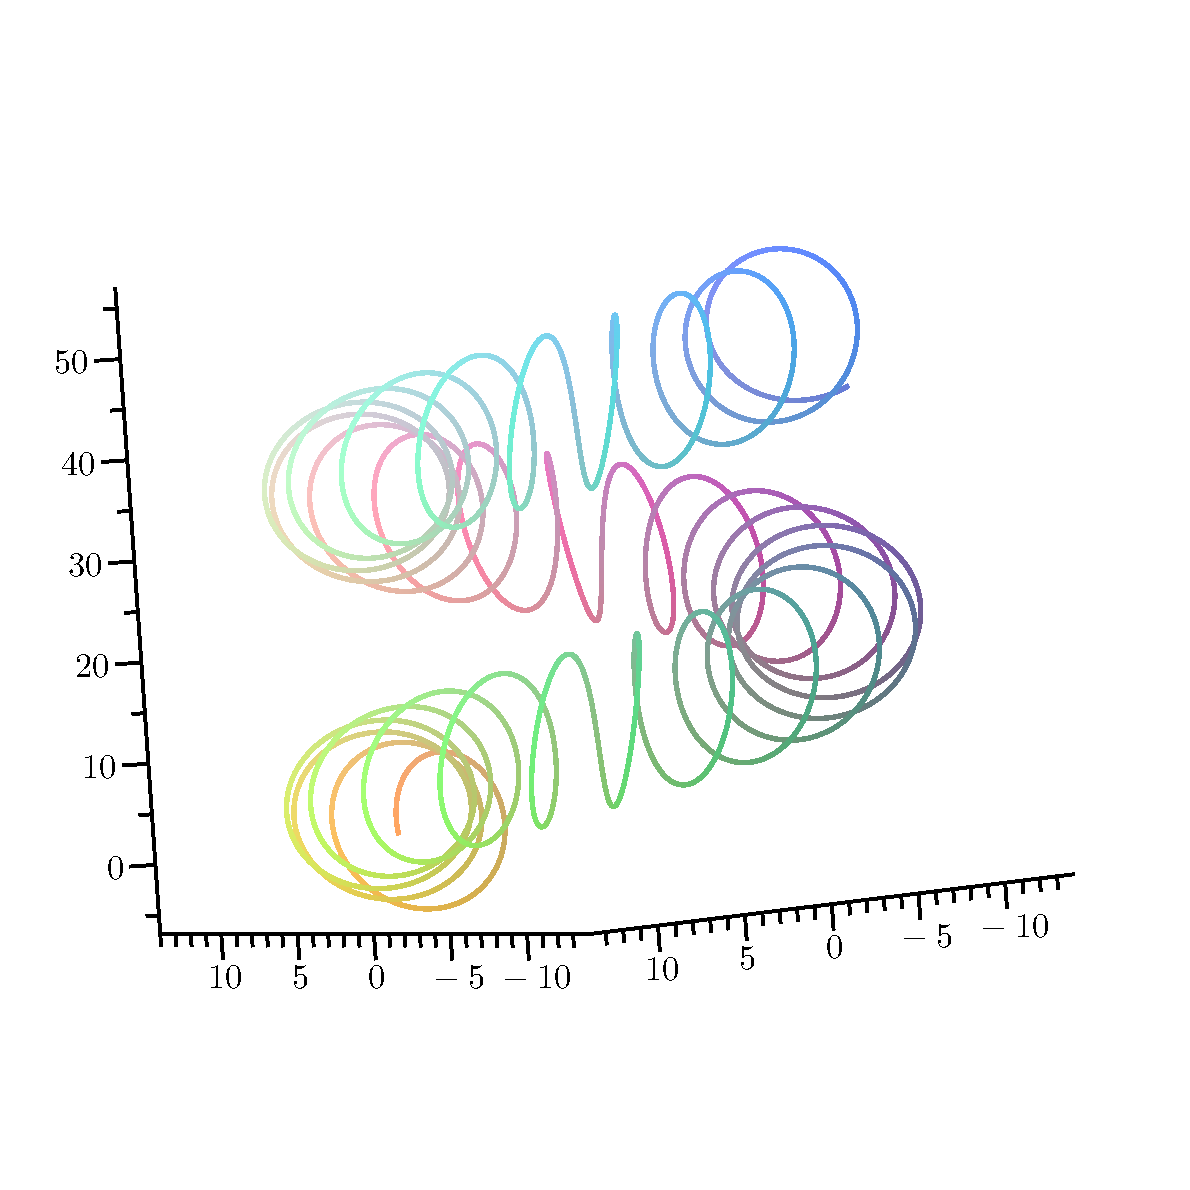
\includegraphics[scale=0.5]{pictures/pureslinky.eps}
\caption{En slinky beskrevet ved \(\gamma(t)=((10+4cos(20t))cos(t), (10+4cos(20t))sin(t), 5t+8sin(20t))\)}
\label{pureslinky}
\end{figure}
\\
For en slinky med samme parameterfremstilling som den vist i figur \ref{pureslinky}, dvs.
\begin{equation}
\begin{gathered}
\gamma(t)=(x(t),y(t),z(t)) \quad t \in [0;10] \\
x(t)=(10+4cos(20t))cos(t) \\
y(t)=(10+4cos(20t))sin(t) \\
z(t)=5t+8sin(20t)
\end{gathered}
\end{equation}
Kurvelængden kan udregnes ved brug af udtrykkene (\ref{Snfinal}) og (\ref{ellnfinal}) for hhv. \(S_n\) og \(\ell_n\). Dette vil vi, ved brug af Maple, gøre for polygonkurver der approksimerer \(\gamma\) med 10, 100 og 1000 hjørnepunkter. De tilhørende Maple-kommandoer ses nedenfor.
\begin{lstlisting}[caption=længden af \(\gamma(t)\) approksimeret med 10 punkter] 
>l:=sum(sqrt((x(t/1)-x((t-1)/1))^2+(y(t/1)-y((t-1)/1))^2+(z(t/1)->z((t-1)/1))^2),t=1..10*1):
evalf(l);
                          117.2099173
>S:=sum(sqrt(D(x)((1+2*n)*1/2)^2+D(y)((1+2*n)*1/2)^2+D(z)((1+2*n)*1/2)^2),n=0..9)*1:
>evalf(S);
                          1222.884938

\end{lstlisting}
\begin{lstlisting}[caption=længden af \(\gamma(t)\) approksimeret med 100 punkter]
>l:=sum(sqrt((x(t/10)-x((t-1)/10))^2+(y(t/10)-y((t-1)/10))^2+(z(t/10)-z((t-1)/10))^2),t=1..10*10):
>evalf(l);
                          1041.639878
>S:=sum(sqrt(D(x)((1+2*n)*0.1/2)^2+D(y)((1+2*n)*0.1/2)^2+D(z)((1+2*n)*0.1/2)^2),n=0..99)*0.1:
>evalf(S);
                          1236.552683

\end{lstlisting}
\begin{lstlisting}[caption=længden af \(\gamma(t)\) approksimeret med 1000 punkter]
>l:=sum(sqrt((x(t/100)-x((t-1)/100))^2+(y(t/100)-y((t-1)/100))^2+(z(t/100)-z((t-1)/100))^2),t=1..10*100):
>evalf(l);
                          1235.332186
>S:=sum(sqrt(D(x)((1+2*n)*0.01/2)^2+D(y)((1+2*n)*0.01/2)^2+D(z)((1+2*n)*0.01/2)^2),n=0..999)*0.01:
>evalf(S);
                          1237.384003

\end{lstlisting}
Udregnes kurvelængden direkte med Maple haves
\begin{lstlisting}[caption=Numerisk evaluering af kurvelængden ved brug af Maples int kommando]
>evalf(int(sqrt((D(x)(t))^2+(D(y)(t))^2+(D(z)(t))^2),t=0..10,numeric=true));
                          1237.390852

\end{lstlisting} 
Det ses at den bedste approksimation for kurvelængden af en slinky klart er \(S_n\), men at \(\ell_n\) dog nærmer sig som \(n\) vokser.  \\
\begin{figure}[hb]
\center
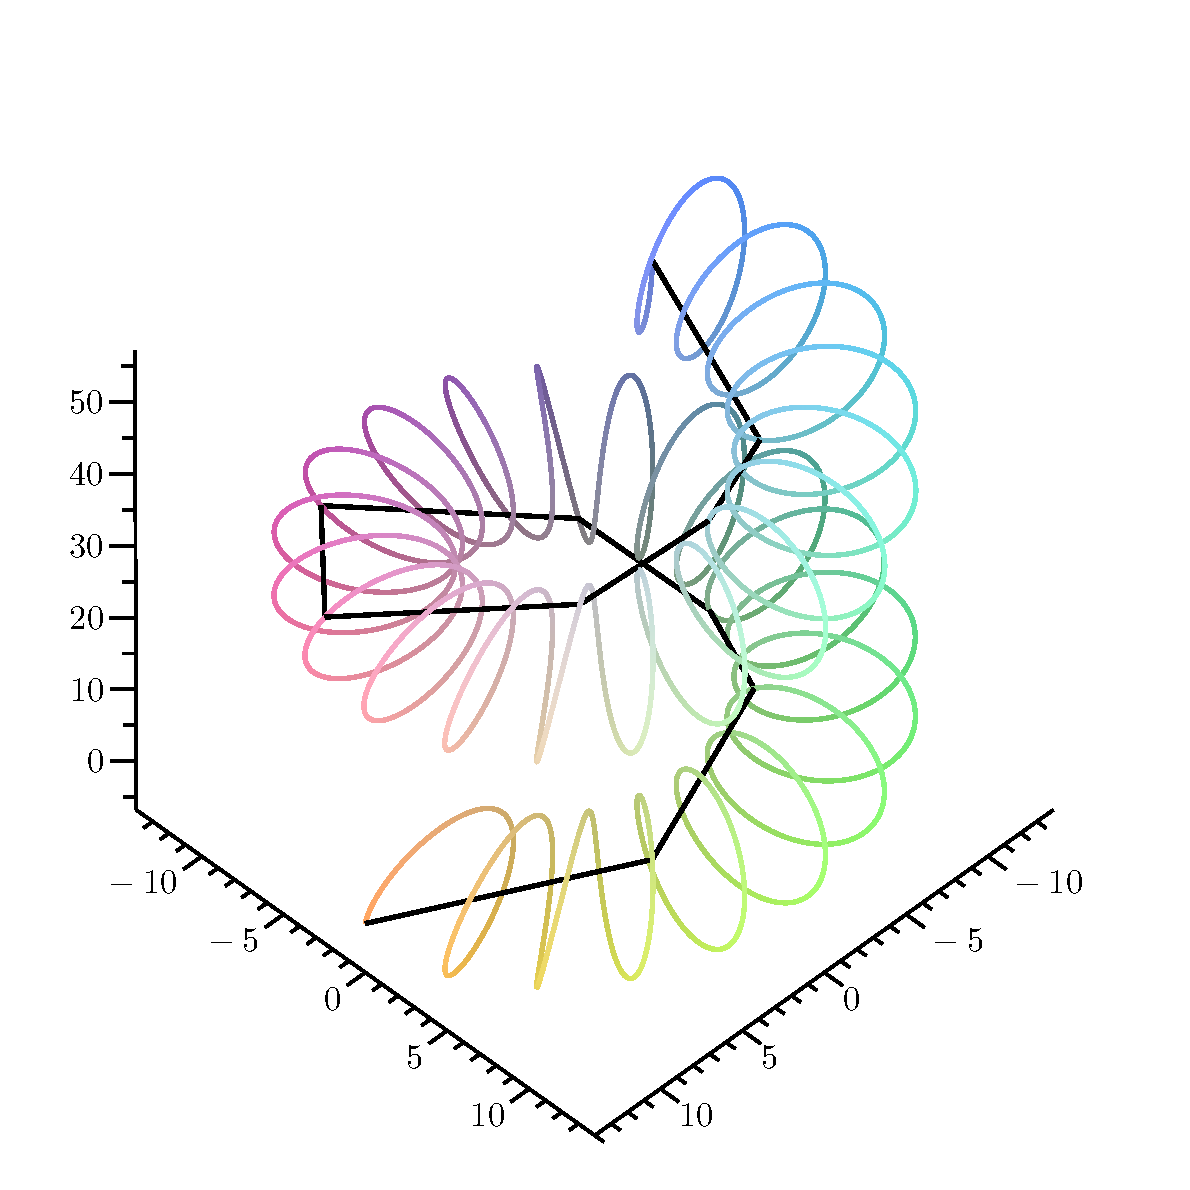
\includegraphics[scale=0.6]{pictures/slinky10.eps}
\caption{Polygonkurven med 10 punkter på \(\gamma\)}
\label{slinky10}
\end{figure}
\begin{figure}[ht]
\center
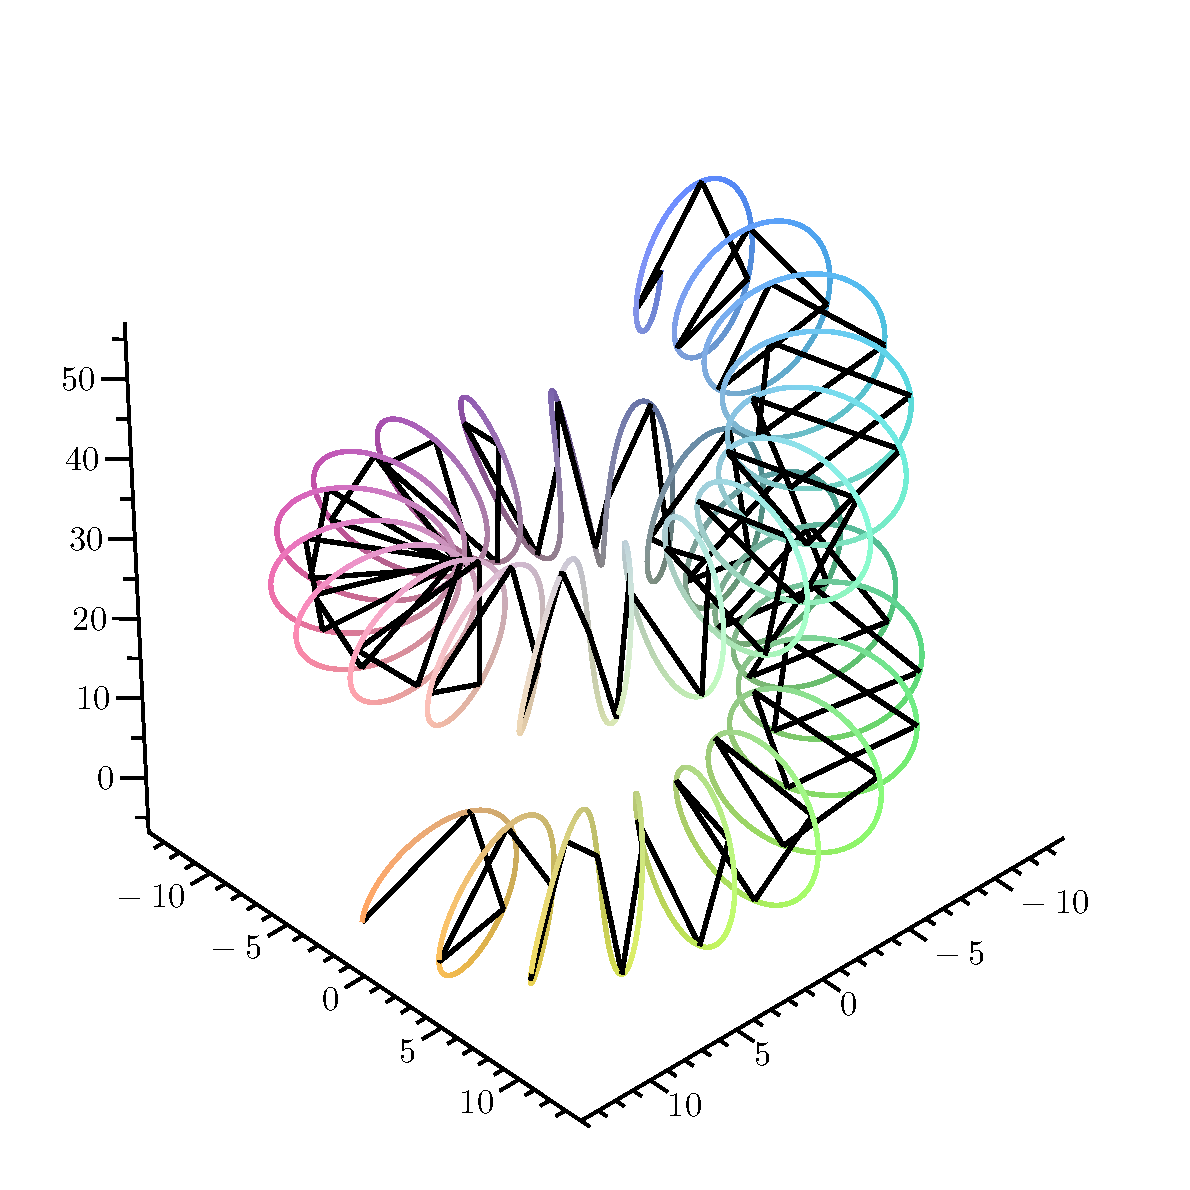
\includegraphics[scale=0.4]{pictures/slinky100.eps}
\caption{Polygonkurven med 100 punkter på \(\gamma\)}
\label{slinky100}
\end{figure}
\begin{figure}[hb]
\center
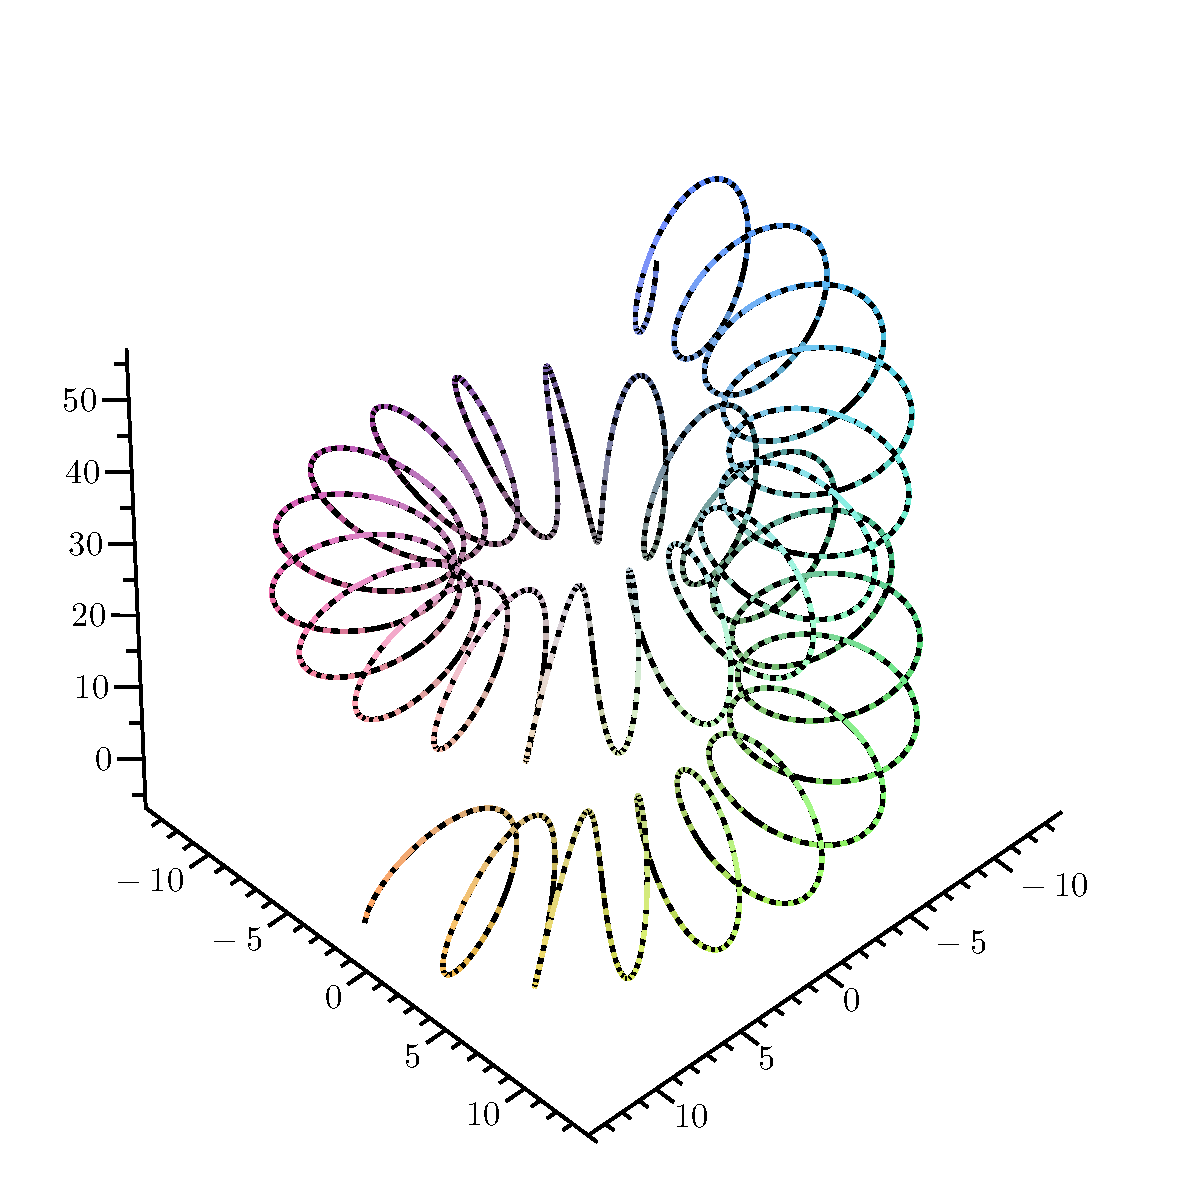
\includegraphics[scale=0.4]{pictures/slinky1000.eps}
\caption{Polygonkurven med 1000 punkter på \(\gamma\)}
\label{slinky1000}
\end{figure}
Det ses på figur \ref{slinky10}, \ref{slinky100} og \ref{slinky1000} at \(\ell_n\) approksimerer \(\pmb{\gamma}(t)\) dårligt for små værdier af \(n\) da polygonkurven tager en smutvej igennem slinkyen. For større \(n\) ses det dog at fejlen bliver mindre da polygonkurven her følger slinkyen rundt i alle dens ringe.
\clearpage
Vi vil nu undersøge om \(S_n\) også er den bedste approksimation for kurverne:
\begin{equation}
\begin{gathered}
\pmb{\gamma}_1(t)=(t^2,t^4,t^6), \quad t\in[-1;1] \\
\pmb{\gamma}_2(t)=(cos(t),sin(t),t), \quad t\in [0;10]
\end{gathered}
\end{equation}
Dog vil vi her nøjes med at kigge på et enkelt antal hjørnepunkter hvor hver polygonkurve. \(\pmb{\gamma}_1(t)\) ses på figur \ref{gamma1graf} og \(\pmb{\gamma}_2(t)\) på figur \ref{gamma2graf}. \\
\begin{figure}[ht]
\center
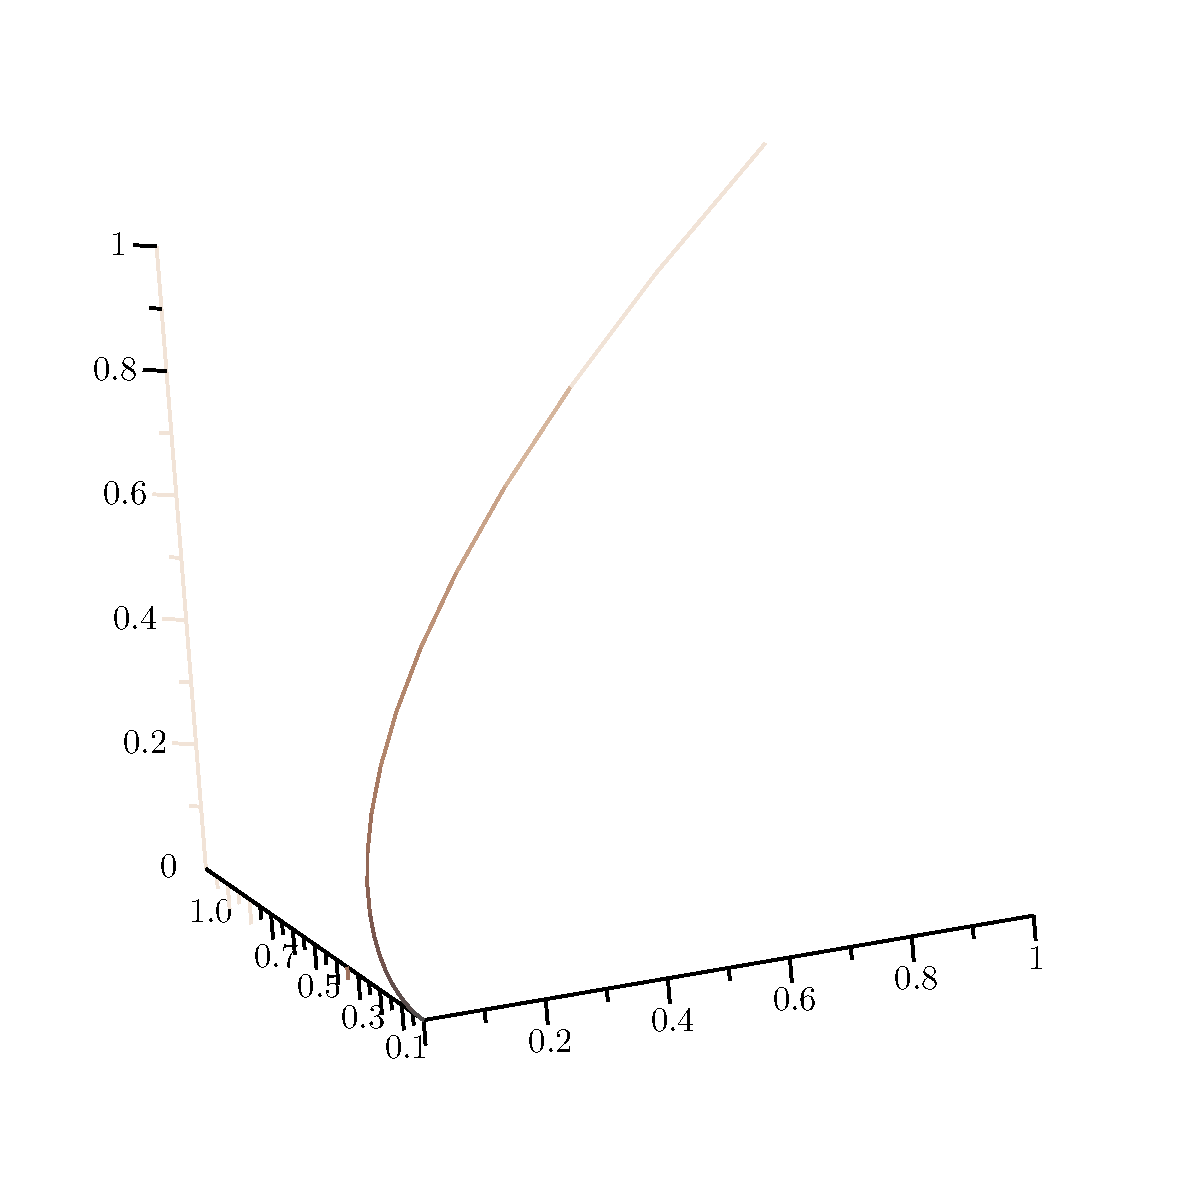
\includegraphics[scale=0.4]{gamma1.eps}
\caption{Afbildning af \(\pmb{\gamma}_1(t)\)}
\label{gamma1graf}
\end{figure}
\begin{figure}[ht]
\center
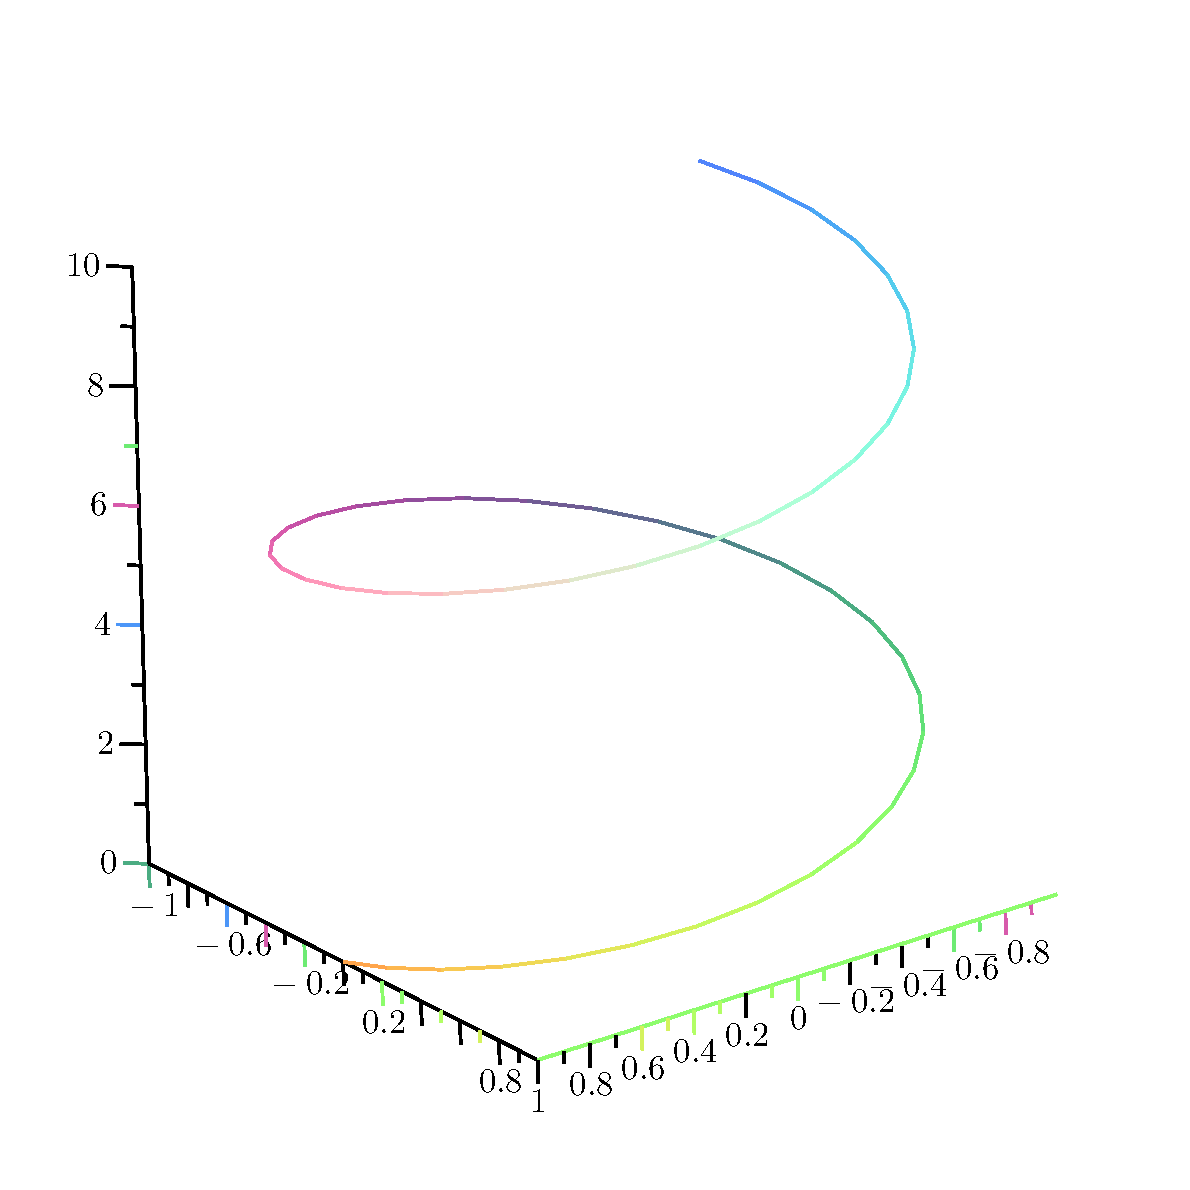
\includegraphics[scale=0.4]{gamma2.eps}
\caption{Afbildning af \(\pmb{\gamma}_2(t)\)}
\label{gamma2graf}
\end{figure}
\\
Udregnes først den numeriske værdi af \(\mathscr{L}(\pmb{\gamma}_1)\) ved hjælp af Maple kommandoen int, til brug som reference for de approksimerende summer, haves:
\begin{lstlisting}[caption=Reference til \(\mathscr{L}(\pmb{\gamma}_1)\)]
>int(sqrt((D(x)(t))^2+(D(y)(t))^2+(D(z)(t))^2),t=-1..1,numeric=true);
                          3.726045965

\end{lstlisting}
Og ved udregning \(S_n,\ell_n\) for en polygonkurve med 200 hjørnepunkter haves
\begin{lstlisting}[caption={Længden af polygonkurven udregnet hvor \( \mbox{l}=\ell_n\) og \(\mbox{S}=S_n\) }]
>l:=sum(sqrt((x((t)/100-1)-x((t-1)/100-1))^2+(y((t)/100-1)-y((t-1)/100-1))^2+(z((t)/100-1)-z((t-1)/100-1))^2),t=1..2*100):
>evalf(l);
                          3.725999606
>S:=sum(sqrt(D(x)(-1+(1+2*n)*0.01/2)^2+D(y)(-1+(1+2*n)*0.01/2)^2+D(z)(-1+(1+2*n)*0.01/2)^2),n=0..199)*0.01:
>evalf(S);
                          3.725804287

\end{lstlisting}
Det ses altså her at \(\ell_n\) er den bedre approksimation \\
\\
For \(\pmb{\gamma}_2(t)\) haves derimod:
\begin{lstlisting}[caption=Reference til \(\mathscr{L}(\pmb{\gamma}_2)\)]
>evalf(int(sqrt((D(x)(t))^2+(D(y)(t))^2+(D(z)(t))^2),t=0..10,numeric=true));
                          14.14213562


\end{lstlisting}
Ved udregning \(S_n,\ell_n\) for en polygonkurve med 1000 hjørnepunkter haves
\begin{lstlisting}[caption={Længden af polygonkurven udregnet hvor \( \mbox{l}=\ell_n\) og \(\mbox{S}=S_n\) }]
>S:=sum(sqrt(D(x)((1+2*n)*0.01/2)^2+D(y)((1+2*n)*0.01/2)^2+D(z)((1+2*n)*0.01/2)^2),n=0..999)*0.01:
>evalf(S);
                          14.14213714
>l:=sum(sqrt((x(t/100)-x((t-1)/100))^2+(y(t/100)-y((t-1)/100))^2+(z(t/100)-z((t-1)/100))^2),t=1..100*10):
>evalf(l);
                          14.14210617

\end{lstlisting}
Her ses det at \(S_n\) er den bedre approksimation af kurvelængden. Kigger vi kun på data fra de foregående 3 eksempler kan vi konkludere at \(S_n\) giver en bedre approksimation når kurven der ønskes approksimeret indeholder repetetive funktioner (\(cos,sin\)), og \(\ell_n\) er den bedre approksimation når kurvens parameterfremstilling er af en højere orden.

\subsection{Polygonkurver som geodæter}